%%%%%%%%%%%%%%%%%%%%%%%%%%%%% Thesis.tex %%%%%%%%%%%%%%%%%%%%%%%%%%%%%%%
%                                                                      %
%  ---------- Master of Science Dissertation template ----------       %
%                                                                      %
%  Template for the Master Thesis according to the regulations         %
%  published by the Academic Board (Direcção Académica) at IST.        %
%                                                                      %
%  For up-to-date guide, please refer to the official website          %
%
% https://tecnico.ulisboa.pt/pt/ensino/estudar-no-tecnico/informacoes-academicas/dissertacao-de-mestrado/
%                                                                      %
%       Andre C. Marta                                                 %
%       Area Cientifica de Mecanica Aplicada e Aeroespacial            %
%       Departamento de Engenharia Mecanica                            %
%       Instituto Superior Tecnico                                     %
%       Av. Rovisco Pais                                               %
%       1049-001 Lisboa                                                %
%       Portugal                                                       %
%       Tel: +351 21 841 9469                                          %
%                        3469 (extension)                              %
%       Email: andre.marta@tecnico.ulisboa.pt                          %
%                                                                      %
%  Created:       Jan 20, 2011                                         %
%  Last Modified: JUn 29, 2022                                         %
%                                                                      %
%%%%%%%%%%%%%%%%%%%%%%%%%%%%%%%%%%%%%%%%%%%%%%%%%%%%%%%%%%%%%%%%%%%%%%%%
%  Revision history                                                    %
%  v1 - 2011/01/24 - original template                                 %
%  v2 - 2012/10/30 - new IST image and glossary support                %
%  v3 - 2013/12/10 - update according to 2012/13 official guide        %
%  v4 - 2014/02/28 - new default for bibliography style                %
%  v5 - 2014/05/07 - update according to 2013/14 official guide        %
%  v6 - 2015/07/02 - cover page format fixed,                          %
%                    contents page numbering fixed,                    %
%                    better language support,                          %
%                    enhanced examples of tables,                      %
%                    new option for appendix page numbering format,    %
%                    custom bibliography style                         %
%  v7 - 2018/02/19 - multiple citations compressed                     %
%  v8 - 2019/05/13 - added examples (pseudo-code)                      %
%  v9 - 2020/03/03 - added French language support                     %
%                    indented first paragraphs                         %
%  v10- 2021/01/29 - place caption above table                         %
%  v11- 2022/06/29 - included Declaration of original work             %
%%%%%%%%%%%%%%%%%%%%%%%%%%%%%%%%%%%%%%%%%%%%%%%%%%%%%%%%%%%%%%%%%%%%%%%%
%                                                                      %
% To generate the PDF file, type "make" at the terminal prompt.        %
%                                                                      %
% The IST template LaTeX package was created by the author             %
% and it can be downloaded from:                                       %
% https://fenix.ist.utl.pt/homepage/ist31052/                          %
%                                                                      %
% The external packages can be downloaded from                         %
% the Comprehensive TeX Archive Network at http://www.ctan.org/        %
%                                                                      %
% List of LaTex symbols:                                               %
% http://www.ctan.org/tex-archive/info/symbols/comprehensive/          %
%                                                                      %
% Help with LaTex can be found at                                      %
% http://www.giss.nasa.gov/tools/latex/ltx-2.html                      %
% http://en.wikibooks.org/wiki/LaTeX                                   %
%%%%%%%%%%%%%%%%%%%%%%%%%%%%%%%%%%%%%%%%%%%%%%%%%%%%%%%%%%%%%%%%%%%%%%%%

%%%%%%%%%%%%%%%%%%%%%%%%%%%%%%%%%%%%%%%%%%%%%%%%%%%%%%%%%%%%%%%%%%%%%%%%
%     Preamble                                                         %
%%%%%%%%%%%%%%%%%%%%%%%%%%%%%%%%%%%%%%%%%%%%%%%%%%%%%%%%%%%%%%%%%%%%%%%%

% ----------------------------------------------------------------------
%  Set the document class
% ----------------------------------------------------------------------
%\renewcommand\bibname{Reference}

\documentclass[10pt,a4paper,twoside]{report}

% ----------------------------------------------------------------------
% Define external packages, language, margins, fonts and new commands
% ----------------------------------------------------------------------
%%%%%%%%%%%%%%%%%%%%%%%%%%%%%%%%%%%%%%%%%%%%%%%%%%%%%%%%%%%%%%%%%%%%%%%%
%                                                                      %
%     File: Thesis_Preamble.tex                                        %
%     Tex Master: Thesis.tex                                           %
%                                                                      %
%     Author: Andre C. Marta                                           %
%     Last modified : 29 Jun 2022                                      %
%                                                                      %
%%%%%%%%%%%%%%%%%%%%%%%%%%%%%%%%%%%%%%%%%%%%%%%%%%%%%%%%%%%%%%%%%%%%%%%%

% 'natbib' package
%
% Flexible bibliography support.
% http://www.ctan.org/tex-archive/macros/latex/contrib/natbib/
%
% > produce author-year style citations
%
% \citet  and \citep  for textual and parenthetical citations, respectively
% \citet* and \citep* that print the full author list, and not just the abbreviated one
% \citealt is the same as \citet but without parentheses. Similarly, \citealp is \citep without parentheses
% \citeauthor
% \citeyear
% \citeyearpar
%
%% natbib options can be provided when package is loaded \usepackage[options]{natbib}
%%
%% Following options are valid:
%%
%%   round  -  round parentheses are used (default)
%%   square -  square brackets are used   [option]
%%   curly  -  curly braces are used      {option}
%%   angle  -  angle brackets are used    <option>
%%   semicolon  -  multiple citations separated by semi-colon (default)
%%   colon  - same as semicolon, an earlier confusion
%%   comma  -  separated by comma
%%   authoryear - for author–year citations (default)
%%   numbers-  selects numerical citations
%%   super  -  numerical citations as superscripts, as in Nature
%%   sort   -  sorts multiple citations according to order in ref. list
%%   sort&compress   -  like sort, but also compresses numerical citations
%%   compress - compresses without sorting
%%
% ******************************* SELECT *******************************
%\usepackage{natbib}          % <<<<< References in alphabetical list Correia, Silva, ...
\usepackage[numbers,sort&compress]{natbib} % <<<<< References in numbered list [1],[2],...
% ******************************* SELECT *******************************


% 'notoccite' package
%
% Prevent trouble from citations in table of contents, etc.
% http://ctan.org/pkg/notoccite
%
% > If you have \cite com­mands in \sec­tion-like com­mands, or in \cap­tion,
%   the ci­ta­tion will also ap­pear in the ta­ble of con­tents, or list of what­ever.
%   If you are also us­ing an un­srt-like bib­li­og­ra­phy style, these ci­ta­tions will
%   come at the very start of the bib­li­og­ra­phy, which is con­fus­ing. This pack­age
%   sup­presses the ef­fect.
%
\usepackage{notoccite}


% ----------------------------------------------------------------------
% Define document language.
% ----------------------------------------------------------------------

% 'inputenc' package
%
% Accept different input encodings.
% http://www.ctan.org/tex-archive/macros/latex/base/
%
% > allows typing non-english text in LaTeX sources.
%
% ******************************* SELECT *******************************
%\usepackage[latin1]{inputenc} % <<<<< Windows
\usepackage[utf8]{inputenc}   % <<<<< Linux
% ******************************* SELECT *******************************


% 'babel' package
%
% Multilingual support for Plain TeX or LaTeX.
% http://www.ctan.org/tex-archive/macros/latex/required/babel/
%
% > sets the variable names according to the language selected
%
% ******************************* SELECT *******************************
%\usepackage[portuguese]{babel} % <<<<< Portuguese
\usepackage[english]{babel} % <<<<< English
%\usepackage[francais]{babel} % <<<<< French (requires package texlive-lang-french)
% ******************************* SELECT *******************************
%\renewcommand{\bibsection}{\chapter*{References}}

% List of LaTeX variable names: \abstractname, \appendixname, \bibname,
%   \chaptername, \contentsname, \listfigurename, \listtablename, ...)
% http://www.tex.ac.uk/cgi-bin/texfaq2html?label=fixnam
%
% Changing the words babel uses (uncomment and redefine as necessary...)
%
\newcommand{\acknowledgments}{@undefined} % new LaTeX variable name
%
% > English
%
\addto\captionsenglish{\renewcommand{\acknowledgments}{Acknowledgments}}
%\addto\captionsenglish{\renewcommand{\contentsname}{Contents}}
%\addto\captionsenglish{\renewcommand{\listtablename}{List of Tables}}
%\addto\captionsenglish{\renewcommand{\listfigurename}{List of Figures}}
%\addto\captionsenglish{\renewcommand{\nomname}{Nomenclature}}
%\addto\captionsenglish{\renewcommand{\glossaryname}{Glossary}}
%\addto\captionsenglish{\renewcommand{\acronymname}{List of Acronyms}}
%\addto\captionsenglish{\renewcommand{\bibname}{References}} % Bibliography
%\addto\captionsenglish{\renewcommand{\appendixname}{Appendix}}

% > French
%
\addto\captionsfrench{\renewcommand{\acknowledgments}{Remerciements}}
%\addto\captionsfrench{\renewcommand{\contentsname}{Table des matières}}
%\addto\captionsfrench{\renewcommand{\listtablename}{Liste des tableaux}}
\addto\captionsfrench{\renewcommand{\listfigurename}{Liste des figures}} % Table des figures
%\addto\captionsfrench{\renewcommand{\nomname}{Nomenclature}}
%\addto\captionsfrench{\renewcommand{\glossaryname}{Glossaire}}
%\addto\captionsfrench{\renewcommand{\acronymname}{Liste des acronymes}}
%\addto\captionsfrench{\renewcommand{\bibname}{Bibliographie}}
%\addto\captionsfrench{\renewcommand{\appendixname}{Annexe}}

% > Portuguese
%
\addto\captionsportuguese{\renewcommand{\acknowledgments}{Agradecimentos}}
%\addto\captionsportuguese{\renewcommand{\contentsname}{Conte\'{u}do}}
%\addto\captionsportuguese{\renewcommand{\listtablename}{Lista de Figuras}}
%\addto\captionsportuguese{\renewcommand{\listfigurename}{Lista de Tabelas}}
\addto\captionsportuguese{\renewcommand{\nomname}{Lista de S\'{i}mbolos}} % Nomenclatura
%\addto\captionsportuguese{\renewcommand{\glossary}{Gloss\'{a}rio}}
%\addto\captionsportuguese{\renewcommand{\acronymname}{Lista de Abrevia\c{c}\~{o}es}}
%\addto\captionsportuguese{\renewcommand{\bibname}{Refer\^{e}ncias}} % Bibliografia
%\addto\captionsportuguese{\renewcommand{\appendixname}{Anexo}} % Apendice


% ----------------------------------------------------------------------
% Define cover fields in both english and portuguese.
% ----------------------------------------------------------------------
%
\newcommand{\coverThesis}{@undefined} % new LaTeX variable name
\newcommand{\coverSupervisors}{@undefined} % new LaTeX variable name
\newcommand{\coverExaminationCommittee}{@undefined} % new LaTeX variable name
\newcommand{\coverChairperson}{@undefined} % new LaTeX variable name
\newcommand{\coverSupervisor}{@undefined} % new LaTeX variable name
\newcommand{\coverMemberCommittee}{@undefined} % new LaTeX variable name
% > English
\addto\captionsenglish{\renewcommand{\coverThesis}{Thesis to obtain the Master of Science Degree in}}
\addto\captionsenglish{\renewcommand{\coverSupervisors}{Supervisor(s)}}
\addto\captionsenglish{\renewcommand{\coverExaminationCommittee}{Examination Committee}}
\addto\captionsenglish{\renewcommand{\coverChairperson}{Chairperson}}
\addto\captionsenglish{\renewcommand{\coverSupervisor}{Supervisor}}
\addto\captionsenglish{\renewcommand{\coverMemberCommittee}{Member of the Committee}}
% > French
\addto\captionsfrench{\renewcommand{\coverThesis}{Th\`ese pour l'obtention du Maîtrise des Sciences en}}
\addto\captionsfrench{\renewcommand{\coverSupervisors}{Directeur(s) de th\`ese}}
\addto\captionsfrench{\renewcommand{\coverExaminationCommittee}{Jury}}
\addto\captionsfrench{\renewcommand{\coverChairperson}{Pr\'esident}}
\addto\captionsfrench{\renewcommand{\coverSupervisor}{Directeur de th\`ese}}
\addto\captionsfrench{\renewcommand{\coverMemberCommittee}{Rapporteur}}
% > Portuguese
\addto\captionsportuguese{\renewcommand{\coverThesis}{Disserta\c{c}\~{a}o para obten\c{c}\~{a}o do Grau de Mestre em}}
\addto\captionsportuguese{\renewcommand{\coverSupervisors}{Orientador(es)}}
\addto\captionsportuguese{\renewcommand{\coverExaminationCommittee}{J\'{u}ri}}
\addto\captionsportuguese{\renewcommand{\coverChairperson}{Presidente}}
\addto\captionsportuguese{\renewcommand{\coverSupervisor}{Orientador}}
\addto\captionsportuguese{\renewcommand{\coverMemberCommittee}{Vogal}}


% ----------------------------------------------------------------------
% Define Declaration of original work in both english and portuguese.
% ----------------------------------------------------------------------
%
\newcommand{\declarationTitle}{@undefined} % new LaTeX variable name
\newcommand{\declarationText}{@undefined}  % new LaTeX variable name
% > English
\addto\captionsenglish{\renewcommand{\declarationTitle}{Declaration}}
\addto\captionsenglish{\renewcommand{\declarationText}{I declare that this document is an original work of my own authorship and that it fulfills all the requirements of the Code of Conduct and Good Practices of the Universidade de Lisboa.}}
% > Portuguese
\addto\captionsportuguese{\renewcommand{\declarationTitle}{Declara\c{c}\~{a}o}}
\addto\captionsportuguese{\renewcommand{\declarationText}{Declaro que o presente documento \'{e} um trabalho original da minha autoria e que cumpre todos os requisitos do C\'{o}digo de Conduta e Boas Pr\'{a}ticas da Universidade de Lisboa.}}


% ----------------------------------------------------------------------
% Define default and cover page fonts.
% ----------------------------------------------------------------------

% Use Arial font as default
%
\renewcommand{\rmdefault}{phv}
\renewcommand{\sfdefault}{phv}

% Define cover page fonts
%
%         encoding     family       series      shape
%  \usefont{T1}     {phv}=helvetica  {b}=bold    {n}=normal
%                   {ptm}=times      {m}=normal  {sl}=slanted
%                                                {it}=italic
% see more examples at
% https://www.overleaf.com/learn/latex/Font_typefaces
% https://tug.org/FontCatalogue/
%
\def\FontLn{% 16 pt normal
  \usefont{T1}{phv}{m}{n}\fontsize{16pt}{16pt}\selectfont}
\def\FontLb{% 16 pt bold
  \usefont{T1}{phv}{b}{n}\fontsize{16pt}{16pt}\selectfont}
\def\FontMn{% 14 pt normal
  \usefont{T1}{phv}{m}{n}\fontsize{14pt}{14pt}\selectfont}
\def\FontMb{% 14 pt bold
  \usefont{T1}{phv}{b}{n}\fontsize{14pt}{14pt}\selectfont}
\def\FontSn{% 12 pt normal
  \usefont{T1}{phv}{m}{n}\fontsize{12pt}{12pt}\selectfont}


% ----------------------------------------------------------------------
% Define page margins and line spacing.
% ----------------------------------------------------------------------

% 'geometry' package
%
% Flexible and complete interface to document dimensions.
% http://www.ctan.org/tex-archive/macros/latex/contrib/geometry/
%
% > set the page margins (2.5cm minimum in every side, as per IST rules)
%
\usepackage{geometry}	
\geometry{verbose,tmargin=2.5cm,bmargin=2.5cm,lmargin=2.5cm,rmargin=2.5cm}

% 'setspace' package
%
% Set space between lines.
% http://www.ctan.org/tex-archive/macros/latex/contrib/setspace/
%
% > allow setting line spacing (line spacing of 1.5, as per IST rules)
%
\usepackage{setspace}
\renewcommand{\baselinestretch}{1.5}


% ----------------------------------------------------------------------
% Define paragraph formating.
% ----------------------------------------------------------------------

% 'indentfirst' package
%
% Indent first paragraph after section header.
% https://ctan.org/pkg/indentfirst
%
% > indent all paragraphs (as per IST rules)
%
\usepackage{indentfirst}	


% ----------------------------------------------------------------------
% Include external packages.
% Note that not all of these packages may be available on all system
% installations. If necessary, include the .sty files locally in
% the <jobname>.tex file directory.
% ----------------------------------------------------------------------

% 'graphicx' package
%
% Enhanced support for graphics.
% http://www.ctan.org/tex-archive/macros/latex/required/graphics/
%
% > extends arguments of the \includegraphics command
%
\usepackage{graphicx}


% 'color' package
%
% Colour control for LaTeX documents.
% http://www.ctan.org/tex-archive/macros/latex/required/graphics/
%
% > defines color macros: \color{<color name>}
%
%\usepackage{color}


% 'amsmath' package
%
% Mathematical enhancements for LaTeX.
% http://www.ctan.org/tex-archive/macros/latex/required/amslatex/
%
% > American Mathematical Society plain Tex macros
%
\usepackage{amsmath}  % AMS mathematical facilities for LaTeX.
\usepackage{amsthm}   % Typesetting theorems (AMS style).
\usepackage{amsfonts} % 


% 'wrapfig' package
%
% Produces figures which text can flow around.
% http://www.ctan.org/tex-archive/macros/latex/contrib/wrapfig/
%
% > wrap figures/tables in text (i.e., Di Vinci style)
%
% \usepackage{wrapfig}


% 'subfigure' package
%
% Deprecated: Figures divided into subfigures.
% http://www.ctan.org/tex-archive/obsolete/macros/latex/contrib/subfigure/
%
% > subcaptions for subfigures
%
\usepackage{subfigure}


% 'subfigmat' package
%
% Automates layout when using the subfigure package.
% http://www.ctan.org/tex-archive/macros/latex/contrib/subfigmat/
%
% > matrices of similar subfigures
%
\usepackage{subfigmat}


% 'url' package
%
% Verbatim with URL-sensitive line breaks.
% http://www.ctan.org/tex-archive/macros/latex/contrib/url/
%
% > URLs in BibTex
%
% \usepackage{url}


% 'varioref' package
%
% Intelligent page references.
% http://www.ctan.org/tex-archive/macros/latex/required/tools/
%
% > smart page, figure, table and equation referencing
%
%\usepackage{varioref}


% 'dcolumn' package
%
% Align on the decimal point of numbers in tabular columns.
% http://www.ctan.org/tex-archive/macros/latex/required/tools/
%
% > decimal-aligned tabular math columns
%
\usepackage{dcolumn}
\newcolumntype{d}{D{.}{.}{-1}} % column aligned by the point separator '.'
\newcolumntype{e}{D{E}{E}{-1}} % column aligned by the exponent 'E'


% 'verbatim' package
%
% Reimplementation of and extensions to LaTeX verbatim.
% http://www.ctan.org/tex-archive/macros/latex/required/tools/
%
% > provides the verbatim environment (\begin{verbatim},\end{verbatim})
%   and a comment environment (\begin{comment},  \end{comment})
%
% \usepackage{verbatim}


% 'moreverb' package
%
% Extended verbatim.
% http://www.ctan.org/tex-archive/macros/latex/contrib/moreverb/
%
% > supports tab expansion and line numbering
%
% \usepackage{moreverb}



% 'nomencl' package
%
% Produce lists of symbols as in nomenclature.
% http://www.ctan.org/tex-archive/macros/latex/contrib/nomencl/
%
% The nomencl package makes use of the MakeIndex program
% in order to produce the nomenclature list.
%
% Nomenclature
% 1) On running the file through LATEX, the command \makenomenclature
%    in the preamble instructs it to create/open the nomenclature file
%    <jobname>.nlo corresponding to the LATEX file <jobname>.tex and
%    writes the information from the \nomenclature commands to this file.
% 2) The next step is to invoke MakeIndex in order to produce the
%    <jobname>.nls file. This can be achieved by making use of the
%    command: makeindex <jobname>.nlo -s nomencl.ist -o <jobname>.nls
% 3) The last step is to invoke LATEX on the <jobname>.tex file once
%    more. There, the \printnomenclature in the document will input the
%    <jobname>.nls file and process it according to the given options.
%
% http://www-h.eng.cam.ac.uk/help/tpl/textprocessing/nomencl.pdf
%
% Nomenclature (produces *.nlo *.nls files)
\usepackage{nomencl}
\makenomenclature
%
% Group variables according to their symbol type
%
\RequirePackage{ifthen} 
\ifthenelse{\equal{\languagename}{english}}%
    { % English
    \renewcommand{\nomgroup}[1]{%
      \ifthenelse{\equal{#1}{R}}{%
        \item[\textbf{Roman symbols}]}{%
        \ifthenelse{\equal{#1}{G}}{%
          \item[\textbf{Greek symbols}]}{%
          \ifthenelse{\equal{#1}{S}}{%
            \item[\textbf{Subscripts}]}{%
            \ifthenelse{\equal{#1}{T}}{%
              \item[\textbf{Superscripts}]}{}}}}}%
    }{%
    \ifthenelse{\equal{\languagename}{french}}%
    { % French
    \renewcommand{\nomgroup}[1]{%
      \ifthenelse{\equal{#1}{R}}{%
        \item[\textbf{Symbole romains}]}{%
        \ifthenelse{\equal{#1}{G}}{%
          \item[\textbf{Symboles grecs}]}{%
          \ifthenelse{\equal{#1}{S}}{%
            \item[\textbf{Indices}]}{% lettre inférieure
            \ifthenelse{\equal{#1}{T}}{%
              \item[\textbf{Exposants}]}{}}}}}% lettre supérieure
    }{ % Portuguese
    \renewcommand{\nomgroup}[1]{%
      \ifthenelse{\equal{#1}{R}}{%
        \item[\textbf{Simbolos romanos}]}{%
        \ifthenelse{\equal{#1}{G}}{%
          \item[\textbf{Simbolos gregos}]}{%
          \ifthenelse{\equal{#1}{S}}{%
            \item[\textbf{Subscritos}]}{%
            \ifthenelse{\equal{#1}{T}}{%
              \item[\textbf{Sobrescritos}]}{}}}}}%
    }}%


% 'glossary' package
%
% Create a glossary.
% http://www.ctan.org/tex-archive/macros/latex/contrib/glossary/
%
% Glossary (produces *.glo *.ist files)
\usepackage[number=none]{glossary}
% (remove blank line between groups)
\setglossary{gloskip={}}
% (redefine glossary style file)
%\renewcommand{\istfilename}{myGlossaryStyle.ist}
\makeglossary


% 'rotating' package
%
% Rotation tools, including rotated full-page floats.
% http://www.ctan.org/tex-archive/macros/latex/contrib/rotating/
%
% > show wide figures and tables in landscape format:
%   use \begin{sidewaystable} and \begin{sidewaysfigure}
%   instead of 'table' and 'figure', respectively.
%
\usepackage{rotating}


% 'hyperref' package
%
% Extensive support for hypertext in LaTeX.
% http://www.ctan.org/tex-archive/macros/latex/contrib/hyperref/
%
% > Extends the functionality of all the LATEX cross-referencing
%   commands (including the table of contents, bibliographies etc) to
%   produce \special commands which a driver can turn into hypertext
%   links; Also provides new commands to allow the user to write adhoc
%   hypertext links, including those to external documents and URLs.
%
\usepackage[pdftex]{hyperref} % enhance documents that are to be
                              % output as HTML and PDF
\hypersetup{colorlinks,       % color text of links and anchors,
                              % eliminates borders around links
%            linkcolor=red,    % color for normal internal links
            linkcolor=black,  % color for normal internal links
            anchorcolor=black,% color for anchor text
%            citecolor=green,  % color for bibliographical citations
            citecolor=black,  % color for bibliographical citations
%            filecolor=magenta,% color for URLs which open local files
            filecolor=black,  % color for URLs which open local files
%            menucolor=red,    % color for Acrobat menu items
            menucolor=black,  % color for Acrobat menu items
%            pagecolor=red,    % color for links to other pages
            pagecolor=black,  % color for links to other pages
%            urlcolor=cyan,    % color for linked URLs
            urlcolor=black,   % color for linked URLs
	          bookmarks=true,         % create PDF bookmarks
	          bookmarksopen=false,    % don't expand bookmarks
	          bookmarksnumbered=true, % number bookmarks
	          pdftitle={Thesis},
            pdfauthor={Andre C. Marta},
            pdfsubject={Thesis Title},
            pdfkeywords={Thesis Keywords},
            pdfstartview=FitV,
            pdfdisplaydoctitle=true}


% 'hypcap' package
%
% Adjusting the anchors of captions.
% http://www.ctan.org/tex-archive/macros/latex/contrib/oberdiek/
%
% > fixes the problem with hyperref, that links to floats points
%   below the caption and not at the beginning of the float.
%
\usepackage[figure,table]{hypcap}


% 'multirow' package
%
% Create tabular cells spanning multiple rows
% http://www.ctan.org/pkg/multirow
%
\usepackage{multirow}


% 'booktabs' package
%
% Publication quality tables in LaTeX
% http://www.ctan.org/pkg/booktabs
%
% > en­hance the qual­ity of ta­bles in LaTeX, pro­vid­ing ex­tra com­mands.
%
% \renewcommand{\arraystretch}{<ratio>} % space between rows
%
\usepackage{booktabs}
%\newcommand{\ra}[1]{\renewcommand{\arraystretch}{#1}}


% 'pdfpages' package
%
% Include PDF documents in LaTeX
% http://www.ctan.org/pkg/pdfpages
%
% > in­clu­sion of ex­ter­nal multi-page PDF doc­u­ments in LaTeX doc­u­ments.
%   Pages may be freely se­lected and sim­i­lar to psnup it is pos­si­ble to put
%   sev­eral log­i­cal pages onto each sheet of pa­per.
%
% \includepdf{filename.pdf}
% \includepdf[pages={4-9},nup=2x3,landscape=true]{filename.pdf}
%
\usepackage{pdfpages}


% 'algorithmicx' package
%
% The algorithmic style you always wanted
% https://ctan.org/pkg/algorithmicx
%
% > provides many possibilities to customizethe layout of algorithms.  You can use one of the predefined layouts(pseudocode,pascalandcand others), with or without modifications,or you can define a completely new layout for your specific needs
%
\usepackage{algorithm}
\usepackage{algpseudocode}


% ----------------------------------------------------------------------
% Define new commands to assure consistent treatment throughout document
% ----------------------------------------------------------------------

\newcommand{\ud}{\mathrm{d}}                % total derivative
\newcommand{\degree}{\ensuremath{^\circ\,}} % degrees

% Abbreviations

\newcommand{\mcol}{\multicolumn}            % table format

\newcommand{\eqnref}[1]{(\ref{#1})}
\newcommand{\class}[1]{\texttt{#1}}
\newcommand{\package}[1]{\texttt{#1}}
\newcommand{\file}[1]{\texttt{#1}}
\newcommand{\BibTeX}{\textsc{Bib}\TeX}

\bibliographystyle{unsrt}

% Typefaces ( example: {\bf Bold text here} )
%
% > pre-defined
%   \bf % bold face
%   \it % italic
%   \tt % typewriter
%
% > newly defined
\newcommand{\tr}[1]{{\ensuremath{\textrm{#1}}}}   % text roman
\newcommand{\tb}[1]{{\ensuremath{\textbf{#1}}}}   % text bold face
\newcommand{\ti}[1]{{\ensuremath{\textit{#1}}}}   % text italic
\newcommand{\mc}[1]{{\ensuremath{\mathcal{#1}}}}  % math calygraphy
\newcommand{\mco}[1]{{\ensuremath{\mathcalold{#1}}}}% math old calygraphy
\newcommand{\mr}[1]{{\ensuremath{\mathrm{#1}}}}   % math roman
\newcommand{\mb}[1]{{\ensuremath{\mathbf{#1}}}}   % math bold face
\newcommand{\bs}[1]{\ensuremath{\boldsymbol{#1}}} % math symbol
\def\bm#1{\mathchoice                             % math bold
  {\mbox{\boldmath$\displaystyle#1$}}%
  {\mbox{\boldmath$#1$}}%
  {\mbox{\boldmath$\scriptstyle#1$}}%
  {\mbox{\boldmath$\scriptscriptstyle#1$}}}
\newcommand{\boldcal}[1]{{\ensuremath{\boldsymbol{\mathcal{#1}}}}}% math bold calygraphy
 % file "Thesis_Preamble.tex"

%%%%%%%%%%%%%%%%%%%%%%%%%%%%%%%%%%%%%%%%%%%%%%%%%%%%%%%%%%%%%%%%%%%%%%%%
%     Begin Document                                                   %
%%%%%%%%%%%%%%%%%%%%%%%%%%%%%%%%%%%%%%%%%%%%%%%%%%%%%%%%%%%%%%%%%%%%%%%%
\begin{document}

% Set plain page style (no headers, footer with centered page number)
\pagestyle{plain}

% Set roman numbering (i,ii,...) before the start of chapters
\pagenumbering{roman}

% ----------------------------------------------------------------------
%  Cover page
% ----------------------------------------------------------------------
%%%%%%%%%%%%%%%%%%%%%%%%%%%%%%%%%%%%%%%%%%%%%%%%%%%%%%%%%%%%%%%%%%%%%%%%
%                                                                      %
%     File: Thesis_FrontCover.tex                                      %
%     Tex Master: Thesis.tex                                           %
%                                                                      %
%     Author: Andre C. Marta                                           %
%     Last modified :  2 Jul 2015                                      %
%                                                                      %
%%%%%%%%%%%%%%%%%%%%%%%%%%%%%%%%%%%%%%%%%%%%%%%%%%%%%%%%%%%%%%%%%%%%%%%%

\thispagestyle {empty}

% IST Logo - Signature A
% parameters: bb=llx lly urx ury (bounding box), width=h_length, height=v_length, angle=angle, scale=factor, clip=true/false, draft=true/false. 

\includegraphics[bb=9.5cm 11cm 0cm 0cm,scale=0.29]{IST_A_CMYK_POS}

\begin{center}
%
% Figure (Image or plot)
\vspace{2.5cm}
% height = 50 mm
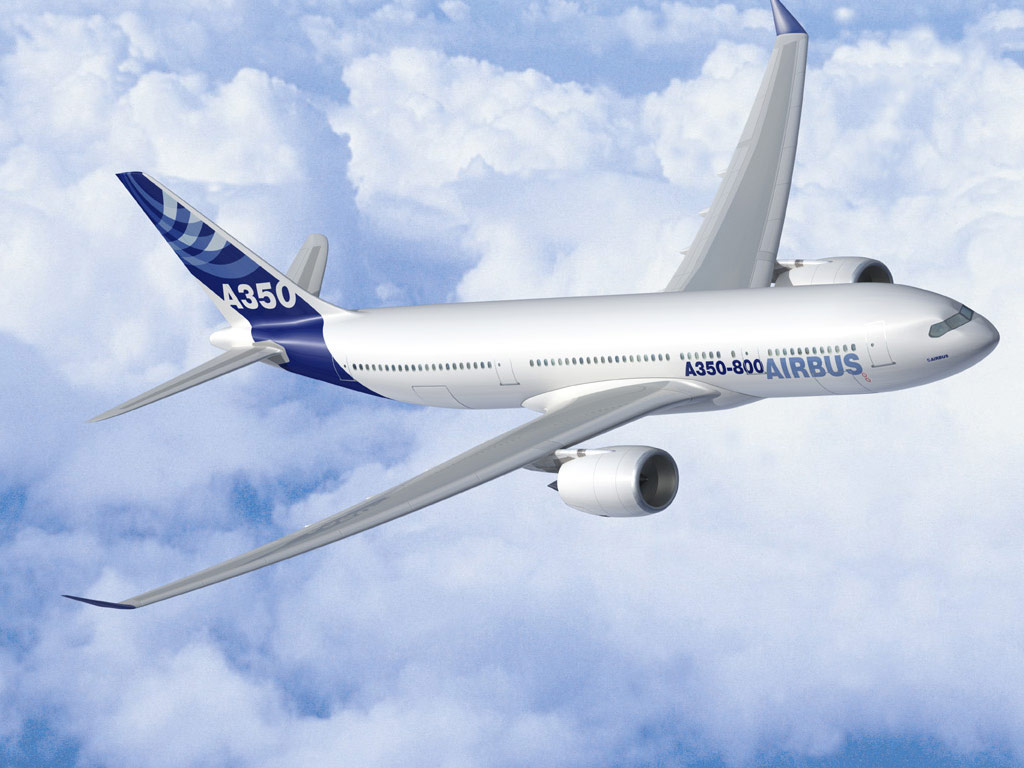
\includegraphics[height=50mm]{Figures/Airbus_A350.jpg}

% Title, author and degree
\vspace{1.0cm}
{\FontLb Thesis Title} \\ % <<<<< EDIT TITLE
%\vspace{0.2cm}
%{\FontMn Subtitle (optional)} \\
%\vspace{1.9cm}
\vspace{2.6cm}
{\FontMb Candidate Full Name} \\ % <<<<< EDIT NAME
\vspace{2.0cm}
{\FontSn \coverThesis} \\
\vspace{0.3cm}
{\FontLb Aerospace Engineering} \\ % <<<<< EDIT COURSE
\vspace{1.0cm}
{\FontSn %
\begin{tabular}{ll}
 \coverSupervisors: & Prof. Full Name 1 \\ % <<<<< EDIT NAME
                    & Dr. Full Name 2    % <<<<< EDIT NAME
\end{tabular} } \\
\vspace{1.0cm}
{\FontMb \coverExaminationCommittee} \\
\vspace{0.3cm}
{\FontSn %
\begin{tabular}{c}
\coverChairperson:     Prof. Full Name          \\ % <<<<< EDIT NAME
\coverSupervisor:      Prof. Full Name 1 (or 2) \\ % <<<<< EDIT NAME
\coverMemberCommittee: Prof. Full Name 3           % <<<<< EDIT NAME
\end{tabular} } \\
\vspace{1.5cm}
{\FontMb Month Year} \\ % <<<<< EDIT DATE (corresponds to date of oral examination)
%
\end{center}

 % file "Thesis_FrontCover.tex"
\clearpage

% ----------------------------------------------------------------------
%  Abstract (both in English and Portuguese)
% ----------------------------------------------------------------------
%%%%%%%%%%%%%%%%%%%%%%%%%%%%%%%%%%%%%%%%%%%%%%%%%%%%%%%%%%%%%%%%%%%%%%%%
%                                                                      %
%     File: Thesis_Abstract.tex                                        %
%     Tex Master: Thesis.tex                                           %
%                                                                      %
%     Author: Andre C. Marta                                           %
%     Last modified :  2 Jul 2015                                      %
%                                                                      %
%%%%%%%%%%%%%%%%%%%%%%%%%%%%%%%%%%%%%%%%%%%%%%%%%%%%%%%%%%%%%%%%%%%%%%%%

\section*{Abstract}

% Add entry in the table of contents as section
\addcontentsline{toc}{section}{Abstract}

Insert your abstract here with a maximum of 250 words, followed by 4 to 6 keywords...

\vfill

\textbf{\Large Keywords:} keyword1, keyword2,...

 % file "Thesis_Abstract.tex"
% \cleardoublepage

% ----------------------------------------------------------------------
%  Table of contents, list of tables, list of figures and nomenclature
% ----------------------------------------------------------------------

% Table of contents
%
\tableofcontents
\cleardoublepage 

% List of tables
%
% Add entry in the table of contents as section
% \phantomsection
% \addcontentsline{toc}{section}{\listtablename}
% Generate list
% \listoftables
% \cleardoublepage 

% List of figures
%
% Add entry in the table of contents as section
% \phantomsection
% \addcontentsline{toc}{section}{\listfigurename}
% Generate list
% \listoffigures
%\cleardoublepage 

% Nomenclature
%
% entries of nomenclature list
% %%%%%%%%%%%%%%%%%%%%%%%%%%%%%%%%%%%%%%%%%%%%%%%%%%%%%%%%%%%%%%%%%%%%%%%%
%                                                                      %
%     File: Thesis_Nomenclature.tex                                    %
%     Tex Master: Thesis.tex                                           %
%                                                                      %
%     Author: Andre C. Marta                                           %
%     Last modified : 29 Jun 2022                                      %
%                                                                      %
%%%%%%%%%%%%%%%%%%%%%%%%%%%%%%%%%%%%%%%%%%%%%%%%%%%%%%%%%%%%%%%%%%%%%%%%
%
% The definitions can be placed anywhere in the document body
% and their order is sorted by <symbol> automatically when
% calling makeindex in the makefile
%
% The \glossary command has the following syntax:
%
% \glossary{entry}
%
% The \nomenclature command has the following syntax:
%
% \nomenclature[<prefix>]{<symbol>}{<description>}
%
% where <prefix> is used for fine tuning the sort order,
% <symbol> is the symbol to be described, and <description> is
% the actual description.

% ----------------------------------------------------------------------
% Roman symbols [r]
\nomenclature[ru]{$\bf u$}{Velocity vector}
\nomenclature[ru]{$u,v,w$}{Velocity Cartesian components}
\nomenclature[rp]{$p$}{Pressure}
\nomenclature[rC]{$C_D$}{Coefficient of drag}
\nomenclature[rC]{$C_L$}{Coefficient of lift}
\nomenclature[rC]{$C_M$}{Coefficient of moment}

% ----------------------------------------------------------------------
% Greek symbols [g]
\nomenclature[g]{$\rho$}{Density}
\nomenclature[g]{$\alpha$}{Angle of attack}
\nomenclature[g]{$\beta$}{Angle of side-slip}
\nomenclature[g]{$\mu$}{Molecular viscosity coefficient}
\nomenclature[g]{$\kappa$}{Thermal conductivity coefficient}

% ----------------------------------------------------------------------
% Subscripts [s]
\nomenclature[s]{$x,y,z$}{Cartesian components}
\nomenclature[s]{$i,j,k$}{Computational indexes}
\nomenclature[s]{$\infty$}{Free-stream condition}
\nomenclature[s]{ref}{Reference condition}
\nomenclature[s]{$n$}{Normal component}

% ----------------------------------------------------------------------
% Supercripts [t]
\nomenclature[t]{T}{Transpose}
\nomenclature[t]{*}{Adjoint}

 % file "Thesis_Nomenclature.tex"
%
% Add entry in the table of contents as section
% \phantomsection
% \addcontentsline{toc}{section}{\nomname}
% Insert glossary/nomenclature section produced by MakeIndex
% \printnomenclature
% \cleardoublepage

% Set arabic numbering (1,2,...) after preface
%
\setcounter{page}{1}
\pagenumbering{arabic}

% ----------------------------------------------------------------------
%  Chapters
% ----------------------------------------------------------------------

%%%%%%%%%%%%%%%%%%%%%%%%%%%%%%%%%%%%%%%%%%%%%%%%%%%%%%%%%%%%%%%%%%%%%%%%
%                                                                      %
%     File: Thesis_Introduction.tex                                    %
%     Tex Master: Thesis.tex                                           %
%                                                                      %
%     Author: Andre C. Marta                                           %
%     Last modified : 13 May 2019                                      %
%                                                                      %
%%%%%%%%%%%%%%%%%%%%%%%%%%%%%%%%%%%%%%%%%%%%%%%%%%%%%%%%%%%%%%%%%%%%%%%%

\chapter{Introduction}
\label{chapter:introduction}

Insert your chapter material here...

%%%%%%%%%%%%%%%%%%%%%%%%%%%%%%%%%%%%%%%%%%%%%%%%%%%%%%%%%%%%%%%%%%%%%%%%
\section{Motivation}
\label{section:motivation}

Relevance of the subject...


%%%%%%%%%%%%%%%%%%%%%%%%%%%%%%%%%%%%%%%%%%%%%%%%%%%%%%%%%%%%%%%%%%%%%%%%
\section{Topic Overview}
\label{section:overview}

Provide an overview of the topic to be studied...


%%%%%%%%%%%%%%%%%%%%%%%%%%%%%%%%%%%%%%%%%%%%%%%%%%%%%%%%%%%%%%%%%%%%%%%%
\section{Objectives and Deliverables}
\label{section:objectives}

Explicitly state the objectives set to be achieved with this thesis...

Also list the expected deliverables.


%%%%%%%%%%%%%%%%%%%%%%%%%%%%%%%%%%%%%%%%%%%%%%%%%%%%%%%%%%%%%%%%%%%%%%%%
\section{Thesis Outline}
\label{section:outline}

Briefly explain the contents of the different chapters...

 % file "Thesis_Introduction.tex"
% \cleardoublepage

\chapter{RISC-V Instruction Set Architecture}
\label{chapter:RISC-V}
\section{RISC-V Overview}
% O que é RISC-V?
% Quais são os ISAs básicos?
RISC-V \cite{RISCV_manual_1}, \cite{RISCV_manual_2} is an instruction set architecture (ISA) that is rapidly growing due to the fact that it is an open-source ISA, contrary to other popular ISAs such as ARM's and Intel's x86. The RISC-V ISA is defined to be a base ISA that is restricted to a minimal set of instructions capable of providing a target to compilers, assemblers, operating systems, etc. In addition to the base ISAs, RISC-V International \cite{RISCV_International} also provides standard extensions and the capability to add custom extensions that enable the developer to add additional capabilities for specific applications.

There are four base ISAs that are characterized by the width of the integer registers and by the number of integer registers. The two primary base ISAs are RV32I and RV64I which provide 32-bit and 64-bit address space, respectively. Both have 32 integer registers. The RV32E is a subset of the RV32I that only has 16 registers and was created to support small microcontrollers. The fourth base ISA is RV128I and supports a 128-bit address space. As mentioned before, RISC-V International provides a few extensions that add some functionalities to the base instruction sets. The most significant among them is the 'M' standard extension that adds integer multiplication and division for signed and unsigned integers. Other extensions are the 'A' standard extension that adds atomic instructions, the 'F' standard extension that provides floating-point operations, floating-point status and control registers and floating-point registers and the 'Zicsr' extension that allows access to the control and status register, this enables interrupt and exception handling.

RISC-V also supports privileged levels and extensions for the privileged ISAs. There are currently three privilege levels: User (U), Supervisor (S) and Machine (M). The privilege modes exist to add protection between components of the software stack. The Machine mode has the most privileges and runs implementation specific firmware. The Supervisor mode is typically used by operating systems and it gives access to most of the hardware. The mode that offers the least privileges is the User mode. It's in this mode that user applications generally run. All implementations must provide the Machine mode since this is the only privileged mode that has access to the entire hardware.

%
%\section{RISC-V Standard Extensions}
% Quais são as extensões que existem?
% Quais são as extensões que preciso?
\section{RISC-V Hardware Implementations}
% O que procuro numa implementação?
% tabela com as implementações que existem
There are many hardware implementations of RISC-V, however, for the purposes of this work, the only implementations analyzed were the ones listed on the list \cite{RISCV_list} under the SoC platforms section, since the focus of this thesis is not to develop the SoC itself. Even though there are several implementations listed it's necessary that the chosen SoC is under an open source license, has good documentation, and an active community support.

Three candidate RISC-V implementations were selected to be studied in detail: LiteX \cite{LiteX}, SweRVolf \cite{SweRVolf} and NEORV32 \cite{NEORV32}. Table \ref{tab:comparação RISC} presents a comparison of the main key factors, such as the base ISA, the supported extensions, the provided RAM size, the system clock speed, the supported simulation tool, and the quality of the documentation provided.

\begin{table}[H]
    \centering
    \begin{tabular}{ c | c | c | c }
         & LiteX & SweRVolf & NEORV32\\
        \hline
        Base ISA & RV32I & RV32I & RV32I\\
        RISC-V Extensions & [M][A][F][D][C] & [M][C] & [M][C][Zicsr][Zicntr]\\ 
        \hline
        RAM & 256MB & 128MB & configurable\\
        system clock & 1MHz & 50MHz & 150MHz\\
        \hline
        Simulation tool & Verilator & Verilator & ISIM\\
        \hline
        Support for RTOS & Zephyr & Zephyr, TockOS & Zephyr, FreeRTOS\\
        \hline
        Documentation & decent & good & decent\\
    \end{tabular}
    \label{tab:comparação RISC}
    \caption{Comparison between RISC-V SoC}
\end{table}

Looking at table \ref{tab:comparação RISC} it's possible to see that the NEORV32 SoC is capable of higher clock speeds and has support for two of more relevant RTOS as will be discussed in Chapter \ref{chapter:RTOS}. However, none of these features is enough to make it the obvious choice, since it also is the more complex one. The LiteX SoC has native support for the Zephyr OS, having a guide on how to install and simulate the RTOS on the Zephyr documentation. The SweRVolf SoC has good support and documentation and already supports relevant RTOS, Zephyr and TockOS. SweRVolf SoC is the SoC selected for this thesis work as it offers resources for the integration of the RTOS that reduces the development effort and ensures a correct integration of the chosen RTOS.

\section{Conclusion}
% Qual é implementação que melhor serve para a tese?
% After analyzing and comparing different RISC-V SoC implementations it can be concluded that the best SoC for this thesis is the SeweRVolf SoC. This is due to the fact that it stands out among the others because of its good support and documentation and its compatibility with relevant RTOS. It offers the necessary computation power with its clock frequency of 50MHz and RAM of 128MB. Besides this, the SoC offers resources for the integration of RTOS that reduce the development effort and ensures a stable integration of the chosen OS.


This chapter provided an overview of the RISC-V ISA. It explained the four base ISA, RV32I, RV64I, RV32E and RV128 as well as some of the more relevant standard extensions. It also introduced the three privilege levels of RISC-V, machine, standard and user. They provide different levels of access to the machine, adding protection between components of the software stack.

A survey of the existing RISC-V hardware implementations was conducted, emphasizing SoC platforms. Of the ones listed in \cite{RISCV_list}, the SoC that were studied in more detail were LiteX, SweRVolf and NEORV32. These implementations were selected based on their open-source license, documentation and community support. Finally, the chosen implementation is SweRVolf as it provides sufficient resources for the installation of the RTOS and offers good documentation and installation guides that will greatly aid the work conducted in this thesis. % file "Thesis_Background_RISC-V.tex"
% \cleardoublepage

\chapter{RTOS Background}
\label{chapter:RTOS}
% \section{Introduction}
% O que é um RTOS?
% Como é que um RTOS funciona internamente?
% Porque é que o RTOS é melhor que GPOS? (fazer a comparação enquanto explico o funcionamento dos RTOS)
\section{RTOS Overview}
A Real-time System is a system where its correctness does not depend only on its output but also depends on the time that the output takes to produce. These systems can be divided into three types: hard real-time systems; soft real-time systems; and firm real-time systems. Hard RTS are those where the system will fail if any task does not finish in its set time. In soft RTS, tasks can fail their time constraints, however, the performance of the overall system can be reduced because of this. Firm RTS have tasks that need to be processed before their deadline, but having some tasks fail that deadline will not make the system fail.

In more complex cases, the use of Operating Systems (OS) is necessary to manage the resources to meet the demands of the system. A Real-time Operating System is an OS designed to take into consideration the necessity of RTS to comply with time constraints. Since an RTOS is an OS it must have some basic functionalities in its kernel such as a process scheduler, memory management, a file system, tasks, multitasking, synchronization, timers and clocks, inter task communication, I/O, and memory management. 

One of the most important capabilities of an OS is its capability to multitask. Since only one task per CPU core can run at any given time, the OS can swap between tasks to improve the system's performance. In those cases, the OS saves the context of the initial task and starts running the highest priority task. Multitasking is especially important in RTOS. When a high priority task is ready to execute it is imperative that the RTOS is able to execute that task so that no time constraint is broken.

In typical RTOS, tasks are grouped into three states: running, ready, and blocked. The running task is the task that is executing on the CPU. Ready tasks are those tasks that are ready to run and are waiting to go to the running state. Finally, the blocked state includes the tasks that cannot run at that moment, usually because they are waiting for an event to occur. When there are multiple tasks ready to be executed the kernel must decide which task is going to use the available resources. In this case, the kernel uses a scheduler. The scheduler is the process that controls which task is running on the CPU at any given time. To execute the tasks, the scheduler makes use of threads. Threads are parts of processes that can run independently of other threads since they have their own stack and registers copy. Threads within the same process also share some resources such as memory and files.

In RTOS, several tasks have to wait for events provided either by other tasks or by the hardware in the system. These events are called interrupts. To handle the interrupts, the RTOS makes use of a mechanism called interrupt service routine (ISR). 



\section{Task Scheduling and Context Switching}
% Como é que as threads functionam num RTOS?
% Como é que o RTOS garante o funcionamento correto das várias tarefas?
The scheduler is the mechanism that is in charge of choosing the task that is executed at any time. The scheduler is especially important in RTOS since it has to ensure that all tasks meet their time constraints. Scheduling algorithms can be divided into two types, preemptive, where the scheduler has the capability to switch the running task even if that task does not go into the blocked state, and cooperative, where the scheduler does not swap the task that is in the running state, but instead, the running task yields the resources periodically. There are a few situations where the scheduler needs to decide what task should run next: when the running task finishes, when the running task moves to the blocked state or when an interrupt happens. In RTOS the most commonly used scheduling algorithms are preemptive, since they provide more control over what task is in the running state.

There are a number of preemptive scheduling algorithms. The most commonly used is priority scheduling or highest priority first. In this scheduling algorithm, every task is assigned a priority. The scheduler then makes sure that the task with the highest priority is always running. If a low priority task is running and a new high priority task goes to the ready state, then that new task starts running and the old task goes to the ready state. Another scheduling algorithms are first come first served, or FIFO, where the selected task is the first task to arrive at the ready state, and shortest job first, where the task with the least amount of computing left executes first. One example of a cooperative scheduling algorithm is round-robin scheduling. With this algorithm the tasks are not assigned any priority, however, the tasks are swapped after a set period of time. It's very common for RTOS to use this type of scheduler to assign running time to tasks of the same priority in priority scheduling.

Another important mechanism of the RTOS is how it handles context switching. Context switching is the mechanism that saves the current state of the task for later use, usually to its stack, and initializes the state of the new running task. This adds overhead that, for RTSs, can make the system fail. That is why it's important that the context switching in RTOS takes as little time as possible. The frequency of context switches depends on the scheduling policy and preemptive scheduling, usually, has more context switches than non-preemptive schedulers. This means that the scheduler has to weigh the context switching delay when choosing what task to execute.




\section{Interrupt Handling}
One of the ways that tasks go from the blocked state to the ready state is when some event occurs. This event can come in the form of software interrupts, such as messages from other tasks, and hardware interrupts, such as input from a keyboard or mouse. To handle the interrupts there is a mechanism called Interrupt Service Routine (ISR). The ISR is a high priority task that runs every time an interrupt occurs and manages the cause of that interrupt. After the triggering of an interrupt, an interrupt request (IRQ) that is associated with the interrupt signals the ISR. The ISR then utilizes an interrupt vector table to determine the correct interrupt handler function. All of this adds a delay which is called interrupt latency. More precisely, interrupt latency is the time between the interrupt signal and the conclusion of the ISR.

Before starting the ISR, the CPU has to save the context of the task it was executing. And after completing the interrupt handling routine the CPU can restore the state it was on or start a new task that was triggered by the interrupt. Sometimes the running thread may need to prevent ISRs from executing, due to some time-sensitive task or critical section operation. In those cases it is possible to disable the ISR, however, this should only be done when no other solution is available, since a more critical task may be delayed because of it.





\section{Resource Sharing}
% Quais são os métodos de comunicaçao entre tarefas?
Since the purpose of the RTOS is to manage and run multiple processes, it's important to mention how the RTOS shares the data and the resources used between the tasks. It's generally unsafe for systems capable of multitasking to access the same data without some kind of protection. Protection may be achieved using the following methods.

\subsection{Temporarily Masking}
Temporarily masking is when the user temporarily disables interrupts and the ability for the kernel to switch tasks. This way the task can process the data knowing that no other tasks will change that data before the processing finishes. Temporarily masking is the fastest way to make sure that the current task has exclusive access to the systems resources, however it should only be used when the longest path through the protected section is smaller then the interrupt latency since this will prevent  any other task from running, even higher priority ones.

\subsection{Semaphores and Mutexes}
A semaphore is an object that controls the access to a specific resource. The semaphore stores how many tasks can access that resource and how many tasks are accessing it at that time. When the number of tasks reaches the limit, no other tasks are allowed to access that resource. This way whenever a task needs to access shared resources it increments the semaphore counter. When that thread finishes it's processing it decreases the semaphore counter. When only one task can access that resource the semaphore is called a binary semaphore.

Similarly to binary semaphores, there is a mechanism called mutex. A mutex ensures mutually exclusive access to a hardware or software resource. When a task wants to access a mutually exclusive resource it must start by locking the associated mutex. After the task is finished it unlocks the locked mutex. While the mutex is locked no other tasks can execute because they cannot access the resources protected by the mutex. The task only starts executing again when the mutex is unlocked. One key difference between mutexes and semaphores is priority inversion. Priority inversion happens when a low priority task locks a mutex and a high priority task is blocked by that mutex. When this happens the priority level of the original task is elevated so that the higher priority task does not have to wait for the low priority task to be assigned CPU time. One problem that comes with mutexes is deadlocking. This happens when, for example, task A locks task B, however, before locking, task B also locked task A. When this happens both tasks are unable to continue executing. This can be prevented by carefully designing the program.

\subsection{Message Passing}
Message passing mechanisms such as FIFOs, stacks, message queues and a mailbox can be used to share data between tasks without the use of shared memory. With this mechanisms a task only shares the data after its processing is done, ensuring that the other tasks only start processing after receiving the data from the first task. Message passing can also make use of priority inversion when a high priority task needs data from a low priority task. Deadlock can also occur when some task is working on data needed for another task, but needs data from the blocked task to continue.


\section{RTOS Comparison}
% Porque é que preciso do RTOS?
% O que é que eu preciso que o RTOS faça?
% tabela de comparação dos RTOS
%In the context of this thesis the RTOS will make use of the previously explained mechanisms to incorporate a hardware accelerator into the system. The RTOS will allow for other tasks to be executed while the accelerator is doing it's work. This allows other tasks to use the CPU resources. When the hardware accelerator finishes some kind of interrupt must be created to inform the system that the swapped thread can continue it's work. The scheduler will also play an important role in the system, since it will be the mechanism that decides what task should run while the accelerator is running and after it finished its work.

Before starting the incorporation of the accelerator into the RTOS it's necessary to choose a reliable RTOS. A series of open source RTOS, seen in \cite{RTOS_List}, were analyzed. Immediately, several of the RTOS in the list were excluded because they either stopped being updated or because they lacked good documentation. After this initial filtering, the RTOS that stood out from the rest were: FreeRTOS \cite{freeRTOS}, RIOT \cite{RIOT} and Zephyr \cite{zephyr}.

\subsection{FreeRTOS}
FreeRTOS is an RTOS that targets small embedded systems. The RTOS has a minimal footprint and prioritizes its small memory size, low overhead, and fast execution. The RTOS Kernel can be tailored to the specific use case of the system with a configuration file called FreeRTOSConfig.h. In addition, its small and simple kernel makes it ideal for systems with limited resources.

Besides the expected capabilities of an RTOS, FreeRTOS also provides some more specific ones. First, it has a very small footprint needing only 4.4 KB of ROM and 500 Bytes of RAM. FreeRTOS has a very fast context switch delay, needing only 84 cycles to swap between tasks. The RTOS uses a highest priority scheduling algorithm, with Round Robin time slicing. Both of these algorithms can be disabled in the configuration file. On top of all this, FreeRTOS also provides excellent documentation and vast community support.

\subsection{RIOT}
RIOT is an RTOS designed to cater to the requirements of Internet of Things devices. The main goal of RIOT is to provide a lightweight but versatile RTOS that runs on a low-power microcontroller but can also use the full power of larger devices with more resources. To achieve this, RIOT uses a modular architecture that allows developers to include only the components needed for the requirements of the system. The programming model is based on event-driven programming. This allows for a highly responsive and efficient system, that still supports multi-tasking. RIOT has a very small footprint requiring only 3.2 KB of ROM and 2.8 KB of RAM. It also has a very small interrupt latency that takes only 50 clock cycles. The RTOS uses a highest priority first scheduling algorithm and a first come first served algorithm for tasks with the same priority.

\subsection{Zephyr}
Zephyr is an RTOS developed by the Linux Foundation. It offers a scalable and secure platform for IoT devices. Similarly to RIOT, it offers a modular architecture that allows for developers to only select the necessary features of the RTOS. This RTOS provides developers a feature rich software that can run in a footprint as small as 8kB and as large as to reach megabytes and supports both 32bit and 64bit architectures.

Besides the expected capabilities of an RTOS, Zephyr offers additional capabilities. First, it has a small footprint, requiring 8 KB of ROM and 4 KB of RAM. It also has a fast context switch delay, taking 264 clock cycles. This RTOS uses a highest priority first scheduler and utilizes the algorithm longest waiting first for tasks of equal priority. It also allows the developer to choose if RTOS will use any time slicing or not. It is also possible to define the task queuing strategies used in the scheduler. 

\subsection{RTOS Feature Comparison}
There are a few characteristics to compare between the RTOS. First, it is important to make sure that the selected RTOS is supported in the chosen SoC, and if not, if the board fits the installation requirements, such as ROM and RAM. It is also important to study how fast can the RTOS process an interrupt and how fast can it switch its context. Finally, it's important to choose an RTOS that has good documentation and strong community support. Table \ref{tab:comparação RTOS} summarizes the characteristics mentioned. Note that some of the more precise metrics, such as interrupt latency and context switch delay, do not have any strict value since they depend on the use case of the RTOS.


% tabela com FreeRTOS, ZephyrOS, RiotOS
\begin{table}[H]
    \centering
    \begin{tabular}{ c | c | c | c }
          & FreeRTOS & RIOT & Zephyr \\ 
        \hline
        Minimum ROM size & 4.4 KB & 3.2 KB & 8 KB\\  
        Minimum RAM size & 500 Bytes & 2.8 KB & 5 KB\\ 
        \hline
        Interrupt Latency & --- & 50 cycles & ---\\
        Context Switch Delay & 84 cycles & --- & 264 cycles \\
        Scheduling Policy & Highest Priority & Highest Priority& Highest Priority\\
        Time Slicing Policy & Round Robin & none & configurable \\
        \hline
        Documentation & Excellent & Good & Excellent\\
    \end{tabular}
    \label{tab:comparação RTOS}
    \caption{Comparison between FreeRTOS, RIOT and Zephyr}
\end{table}

Looking at the metrics mentioned in Table \ref{tab:comparação RTOS}, t it's possible to see that FreeRTOS should perform better for smaller systems that have less RAM and ROM available. It is also a better RTOS when dealing with small tasks and the context switch delay is more impactful. At the same time, due to its vast variety of capabilities, it's possible to conclude that ZephyrOS should perform better for larger systems. In this system the context switch delay should not be as impactful, making the pros of the RTOS outweigh the cons. The support for the chosen SoC is also an important feature to consider. None of the RTOS analyzed have direct support in their documentation page, however, both FreeRTOS and Zephyr have online guides on how to use them with the chosen SoC, SweRVolfX. 

Since ZephyrOS is the RTOS with better support and documentation it will be the one used. However, it's important to keep in mind that, if the capabilities provided are not useful or even worsen the performance of the overall system, the lighter option should be used.


\section{Conclusion}
This Chapter provides an overview of RTOS. It explains the different types of RTS: hard, soft, and firm real-time systems. It also explains how the performance of those systems varies with the correctness of the time constraints. After that, it summarizes how the RTOS manages the different tasks making use of the scheduler and context switching. It also describes some of the most common preemptive scheduling algorithms: priority scheduling, first come first served, and shortest job first. After that, it explains how an RTOS makes use of the ISR to handle interrupts. The last mechanisms of a RTOS summarized in this Chapter are the ones used for resource sharing. This includes temporarily masking, Semaphores, Mutexes, and message-passing mechanisms.

Finally, this chapter provides a comparison between three RTOS: FreeRTOS, RIOT and Zephyr. To select the RTOS used for this thesis some characteristics of the RTOS were analyzed. First, there are some more technical characteristics that are important such as the minimum ROM and RAM size that they need, the interrupt latency, the context switch delay, and the scheduling policies used. Since all the RTOS provide the necessary capabilities for this thesis work, the decision was made based on the documentation and community support that each RTOS provides. In this field, ZephyrOS is the best candidate.







%Detalhar o kernel
%Mecanismos especificos do rtos
%Como é que o rtos gere/cria as threads e como é que é difere do gpos
%Tabela de comparação
%Conclusões


% na introdução falar mais de threads % file "Thesis_Background_RTOS.tex"
% \cleardoublepage

\chapter{RVfpga}
\label{chapter:rvfpga}
\section{Baseline SoC: RVfpgaNexys}
In section \ref{section:RISCV}, after analyzing several different RISC-V based SoCs, the SweRVolf SoC was chosen as the baseline SoC for this thesis. RVfpgaNexys is an extended version of SweRVolf targeted to the Nexys A7 board. The extended SweRVolf, or SweRVolfX, adds 4 peripherals to SweRVolf: a GPIO interface for the board's LEDs and switches, a PTC, an additional SPI, and a controller for the 8 digit 7-Segment Displays.

\begin{figure}[h]
    \centering
    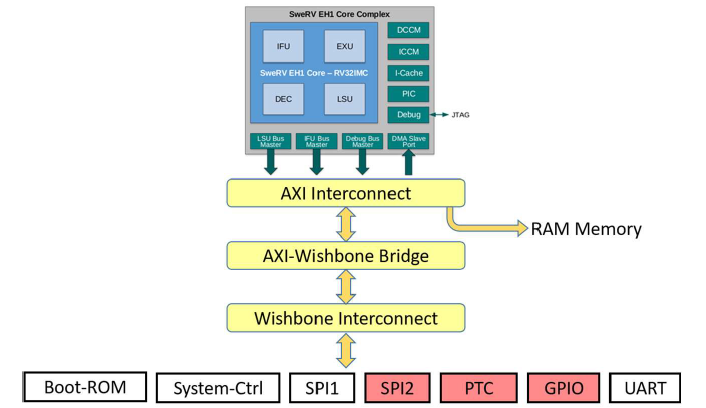
\includegraphics[scale=0.7]{Figures/SweRVolfX.png}
    \caption{SweRVolfX block diagram from Imagination Technologies}
    \label{fig:SweRVolfX}
\end{figure}

Figure \ref{fig:SweRVolfX} shows the block diagram of the SweRVolfX SoC. The SoC utilizes the SweRV EH1 Core Complex from Western DIgital with a 32-bit (RV32ICM) core. The SweRVolf SoC includes a Boot ROM, UART, a System Controller and an SPI controller. The peripherals use a Wishbone bus, however the SweRV EH1 Core uses AXI, so the SoC also includes a AXI to Wishbone bridge. The RAM memory is connected to the processor through the AXI interconnect.

\begin{figure}[H]
    \centering
    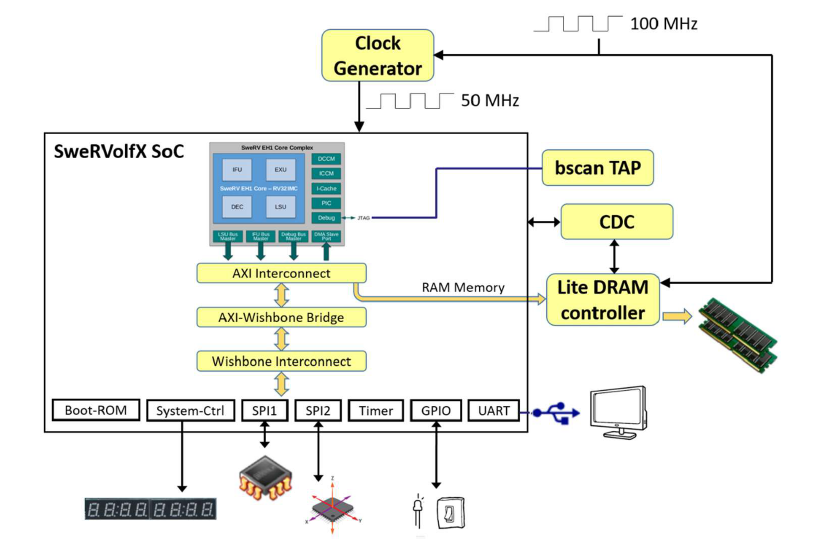
\includegraphics[scale=0.5]{Figures/RVfpgaNexys.png}
    \caption{RVfpgaNexys block diagram from Imagination Technologies}
    \label{fig:RVfpgaNexys}
\end{figure}

Figure \ref{fig:RVfpgaNexys} has a block diagram that shows how the SweRVolfX SoC and the Nexys A7 board interact with each other.

TODO Recursos utilizados pela SoC
TODO Benchmarks corridos

\section{AXI Interconnect}
TODO Explicar AXI Interconnect
TODO O que é preciso adicionar?
TODO Primeiro tentei modificar o interconnect que já lá estava. Porque não funcionou?
TODO Depois tentei utilizar uma opção open source para manter a SoC completamente simulável e open source. Porque é que não deu?
TODO Finalmente utilizei o AXI interconnect da xilinx. Porque foi a melhor opção?
TODO Quais são os ports que lá estão e para que servem?
TODO Recursos utilizados pela SoC e comparar com a versão anterior
TODO Benchmarks corridos e comparar com a versão anterior

\section{Hardware Accelerator}
TODO Explicar acelerador
TODO Qual é o funcionamento básico do acelerador?
TODO Como o desenhei no HLS? Quais foram os recursos utilizados para o acelerador?
TODO Como é que a SoC interaje com o acelerador?
TODO Recursos utilizados pela SoC e comparar com a versão anterior
TODO Benchmarks corridos e comparar com a versão anterior % file "Thesis_RVfpga.tex"


%%%%%%%%%%%%%%%%%%%%%%%%%%%%%%%%%%%%%%%%%%%%%%%%%%%%%%%%%%%%%%%%%%%%%%%%
%                                                                      %
%     File: Thesis_Conclusions.tex                                     %
%     Tex Master: Thesis.tex                                           %
%                                                                      %
%     Author: Andre C. Marta                                           %
%     Last modified :  2 Jul 2015                                      %
%                                                                      %
%%%%%%%%%%%%%%%%%%%%%%%%%%%%%%%%%%%%%%%%%%%%%%%%%%%%%%%%%%%%%%%%%%%%%%%%

\chapter{Conclusions}
\label{chapter:conclusions}

Insert your chapter material here...


% ----------------------------------------------------------------------
\section{Achievements}
\label{section:achievements}

The major achievements of the present work...


% ----------------------------------------------------------------------
\section{Future Work}
\label{section:future}

A few ideas for future work...

 % file "Thesis_Conclusions.tex"
% \cleardoublepage

% ----------------------------------------------------------------------
%  Bibliography
% ----------------------------------------------------------------------

% Add entry in the table of contents as chapter
\phantomsection
\renewcommand\bibname{References}
\addcontentsline{toc}{chapter}{\bibname}

% Custom bibliography style adapted from 'natbib' package
%   (based on http://tex.stackexchange.com/questions/5053/is-it-possible-to-get-unsrt-abbrv-bibliography)
%   (unsrtnat.bst + abbrvnat.bst -> abbrvunsrtnat.bst)
%   (original files copied from:
%   http://tug.ctan.org/macros/latex/contrib/natbib/abbrvnat.bst
%   http://tug.ctan.org/macros/latex/contrib/natbib/unsrtnat.bst
% > unsorted with entries appearing in the order in which the citations appear, with first names and names of journals and months abbreviated.
\bibliographystyle{unsrtnat} % <<<<< SELECT IF USING REFERENCES BY NUMBER (CITATION ORDER)

% External bibliography database file in the BibTeX format
\bibliography{Thesis_bib_DB} % file "Thesis_bib_DB.bib"

% ----------------------------------------------------------------------
\end{document}
% ----------------------------------------------------------------------

